\chapter{Patrones Creacionales}
\section{Introducción}
contenido...
\newpage

\section{Singleton}

\subsection{Realización}
\begin{figure}[h!]
	\centering
	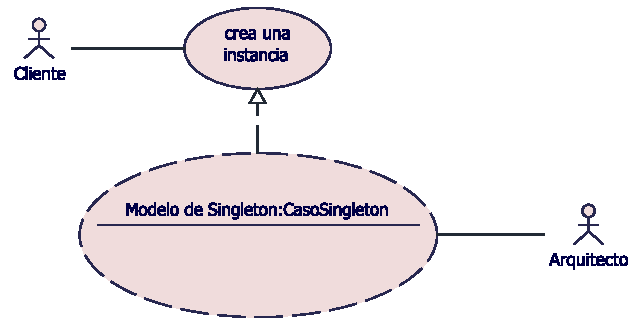
\includegraphics[width=0.7\linewidth]{PATRONES/imgs/MRSingleton}
	\caption{Realizacion de Singleton}
	\label{fig:mrsingleton}
\end{figure}

\subsection{Modelo}
\begin{figure}[h!]
	\centering
	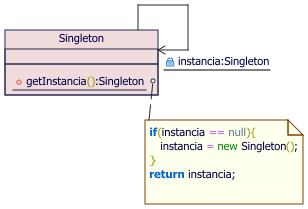
\includegraphics[width=0.7\linewidth]{PATRONES/imgs/MCSingleton}
	\caption{Realizacion de Singleton}
	\label{fig:mrsingleton}
\end{figure}
\subsection{Implementación}
\begin{figure}[h!]
	\centering
	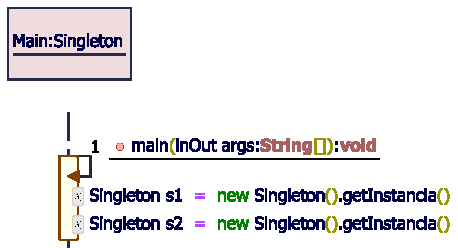
\includegraphics[width=0.7\linewidth]{PATRONES/imgs/MISingleton}
	\caption{Realizacion de Singleton}
	\label{fig:mrsingleton}
\end{figure}
\newpage
\lstinputlisting[caption=Sinlgeton]{c:/a/Singleton.java}

\subsection{Fuentes}